El diseño final del circuito se muestra en la figura \ref{fig:final-design}:

\begin{figure}[H]
  \centering
  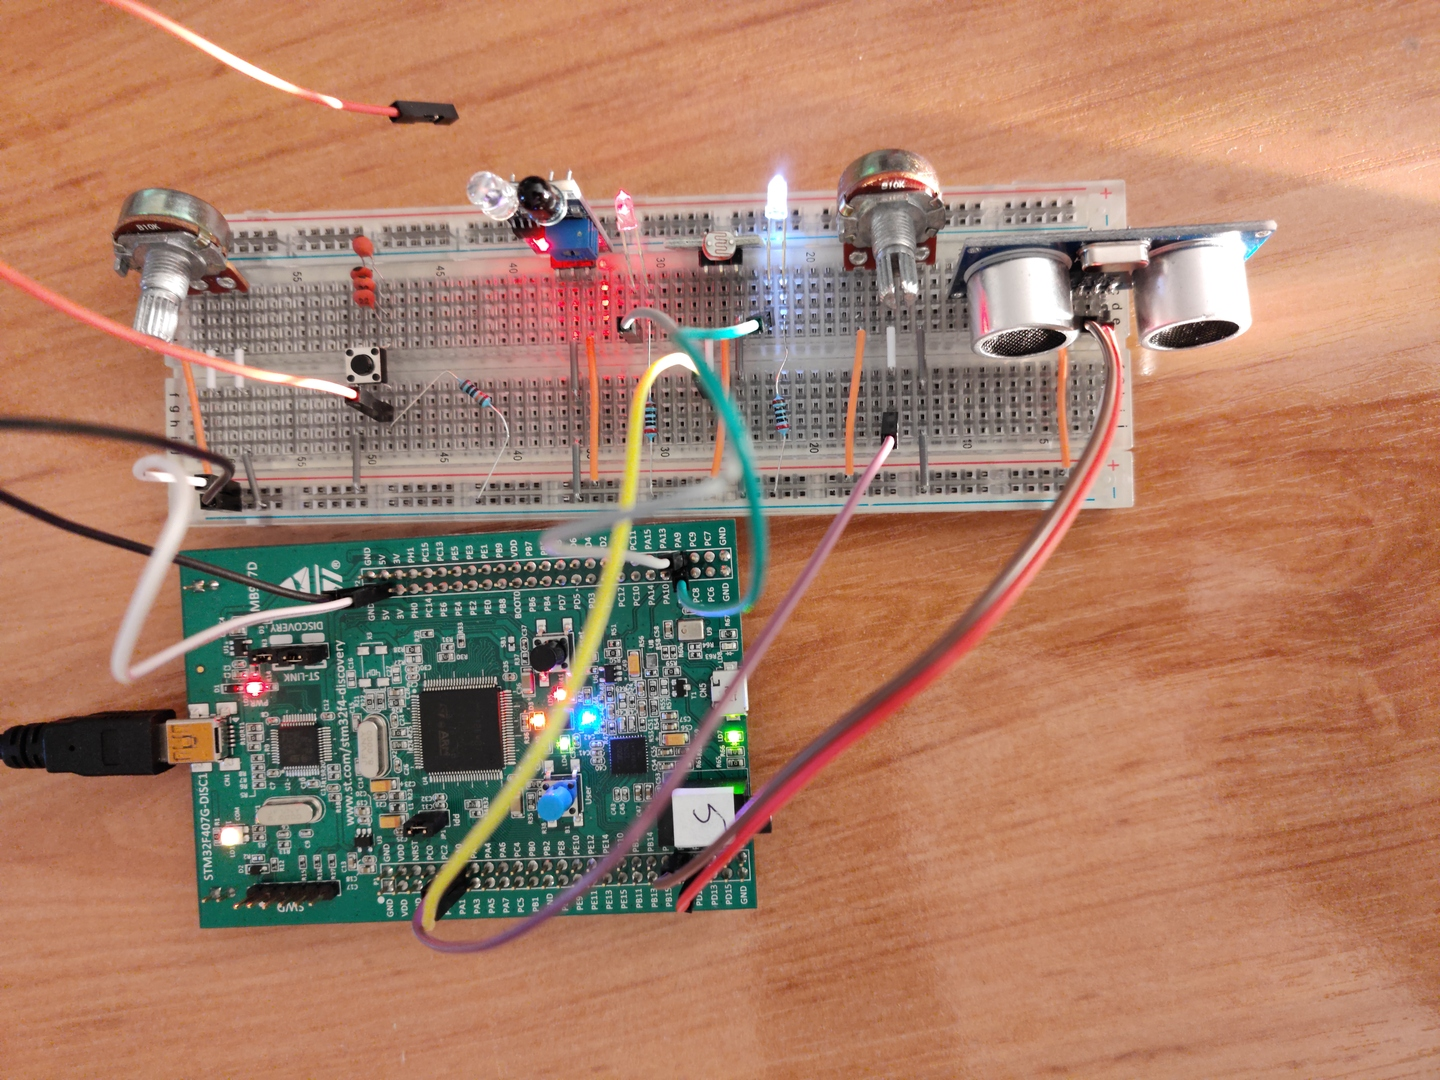
\includegraphics[width=\linewidth]{pictures/final-design.lq.jpg}
  \caption{Diseño final del circuito montado sobre una \textit{protoboard}.}
  \label{fig:final-design}
\end{figure}

Como se puede ver en la figura anterior, todo el circuito (de los dos nodos)
se ha podido montar sobre la misma placa de desarrollo: se pueden apreciar los
dos potenciómetros (volante y acelerador), el sensor de presencia para el agarre
del volante, LDR para luz ambiental, múltiples LEDs para mostrar señales, etc.

Con el código implementado se ha conseguido que las tareas funcionen como se esperaban
y que se puedan realizar algunas comunicaciones mediante el CANBus. Sin embargo, la
falta de tiempo (e inexperiencia del equipo) durante el desarrollo del proyecto ha
dejado \textit{bugs} sin resolver y el código no está todo lo depurado que
convendría para un sistema en tiempo real.

Por otra parte, y en estrecha relación con lo mencionado anteriormente, solo se
han podido implementar dos nodos, teniendo que postergar el desarrollo del nodo
\textit{display} para otro momento.

Finalmente, se asume que el sistema es planificable ya que los accesos a CPU y
recursos no son tan grandes como para que alguna tarea saliese no planificable.
Sin embargo, sería interesante poder realizar observaciones y mediciones sobre
un prototipo en avanzado estado de desarrollo para extraer el WCET $C_i$ de
cada tarea, realizar el RTA (\textit{Response Time Analysis}) y verificar que
efectivamente el sistema es planificable o, en otro caso, realizar los ajustes
pertinentes para que lo sea.